\chapter{Реализация и тестирование программного комплекса}
\label{ch:implementation}

\section{Реализация пользовательского интерфейса}

Пользовательский интерфейс (GUI) является точкой входа для взаимодействия пользователя с системой. Он спроектирован с упором на простоту, наглядность и отзывчивость. Основой для реализации послужила библиотека Fyne. Главное окно приложения состоит из контейнера с вкладками (\texttt{container.NewAppTabs}), который организует основной функционал по четырем направлениям: «Мониторинг», «Производительность», «Память» и «Многозадачность».

\begin{figure}[ht!]
\centering
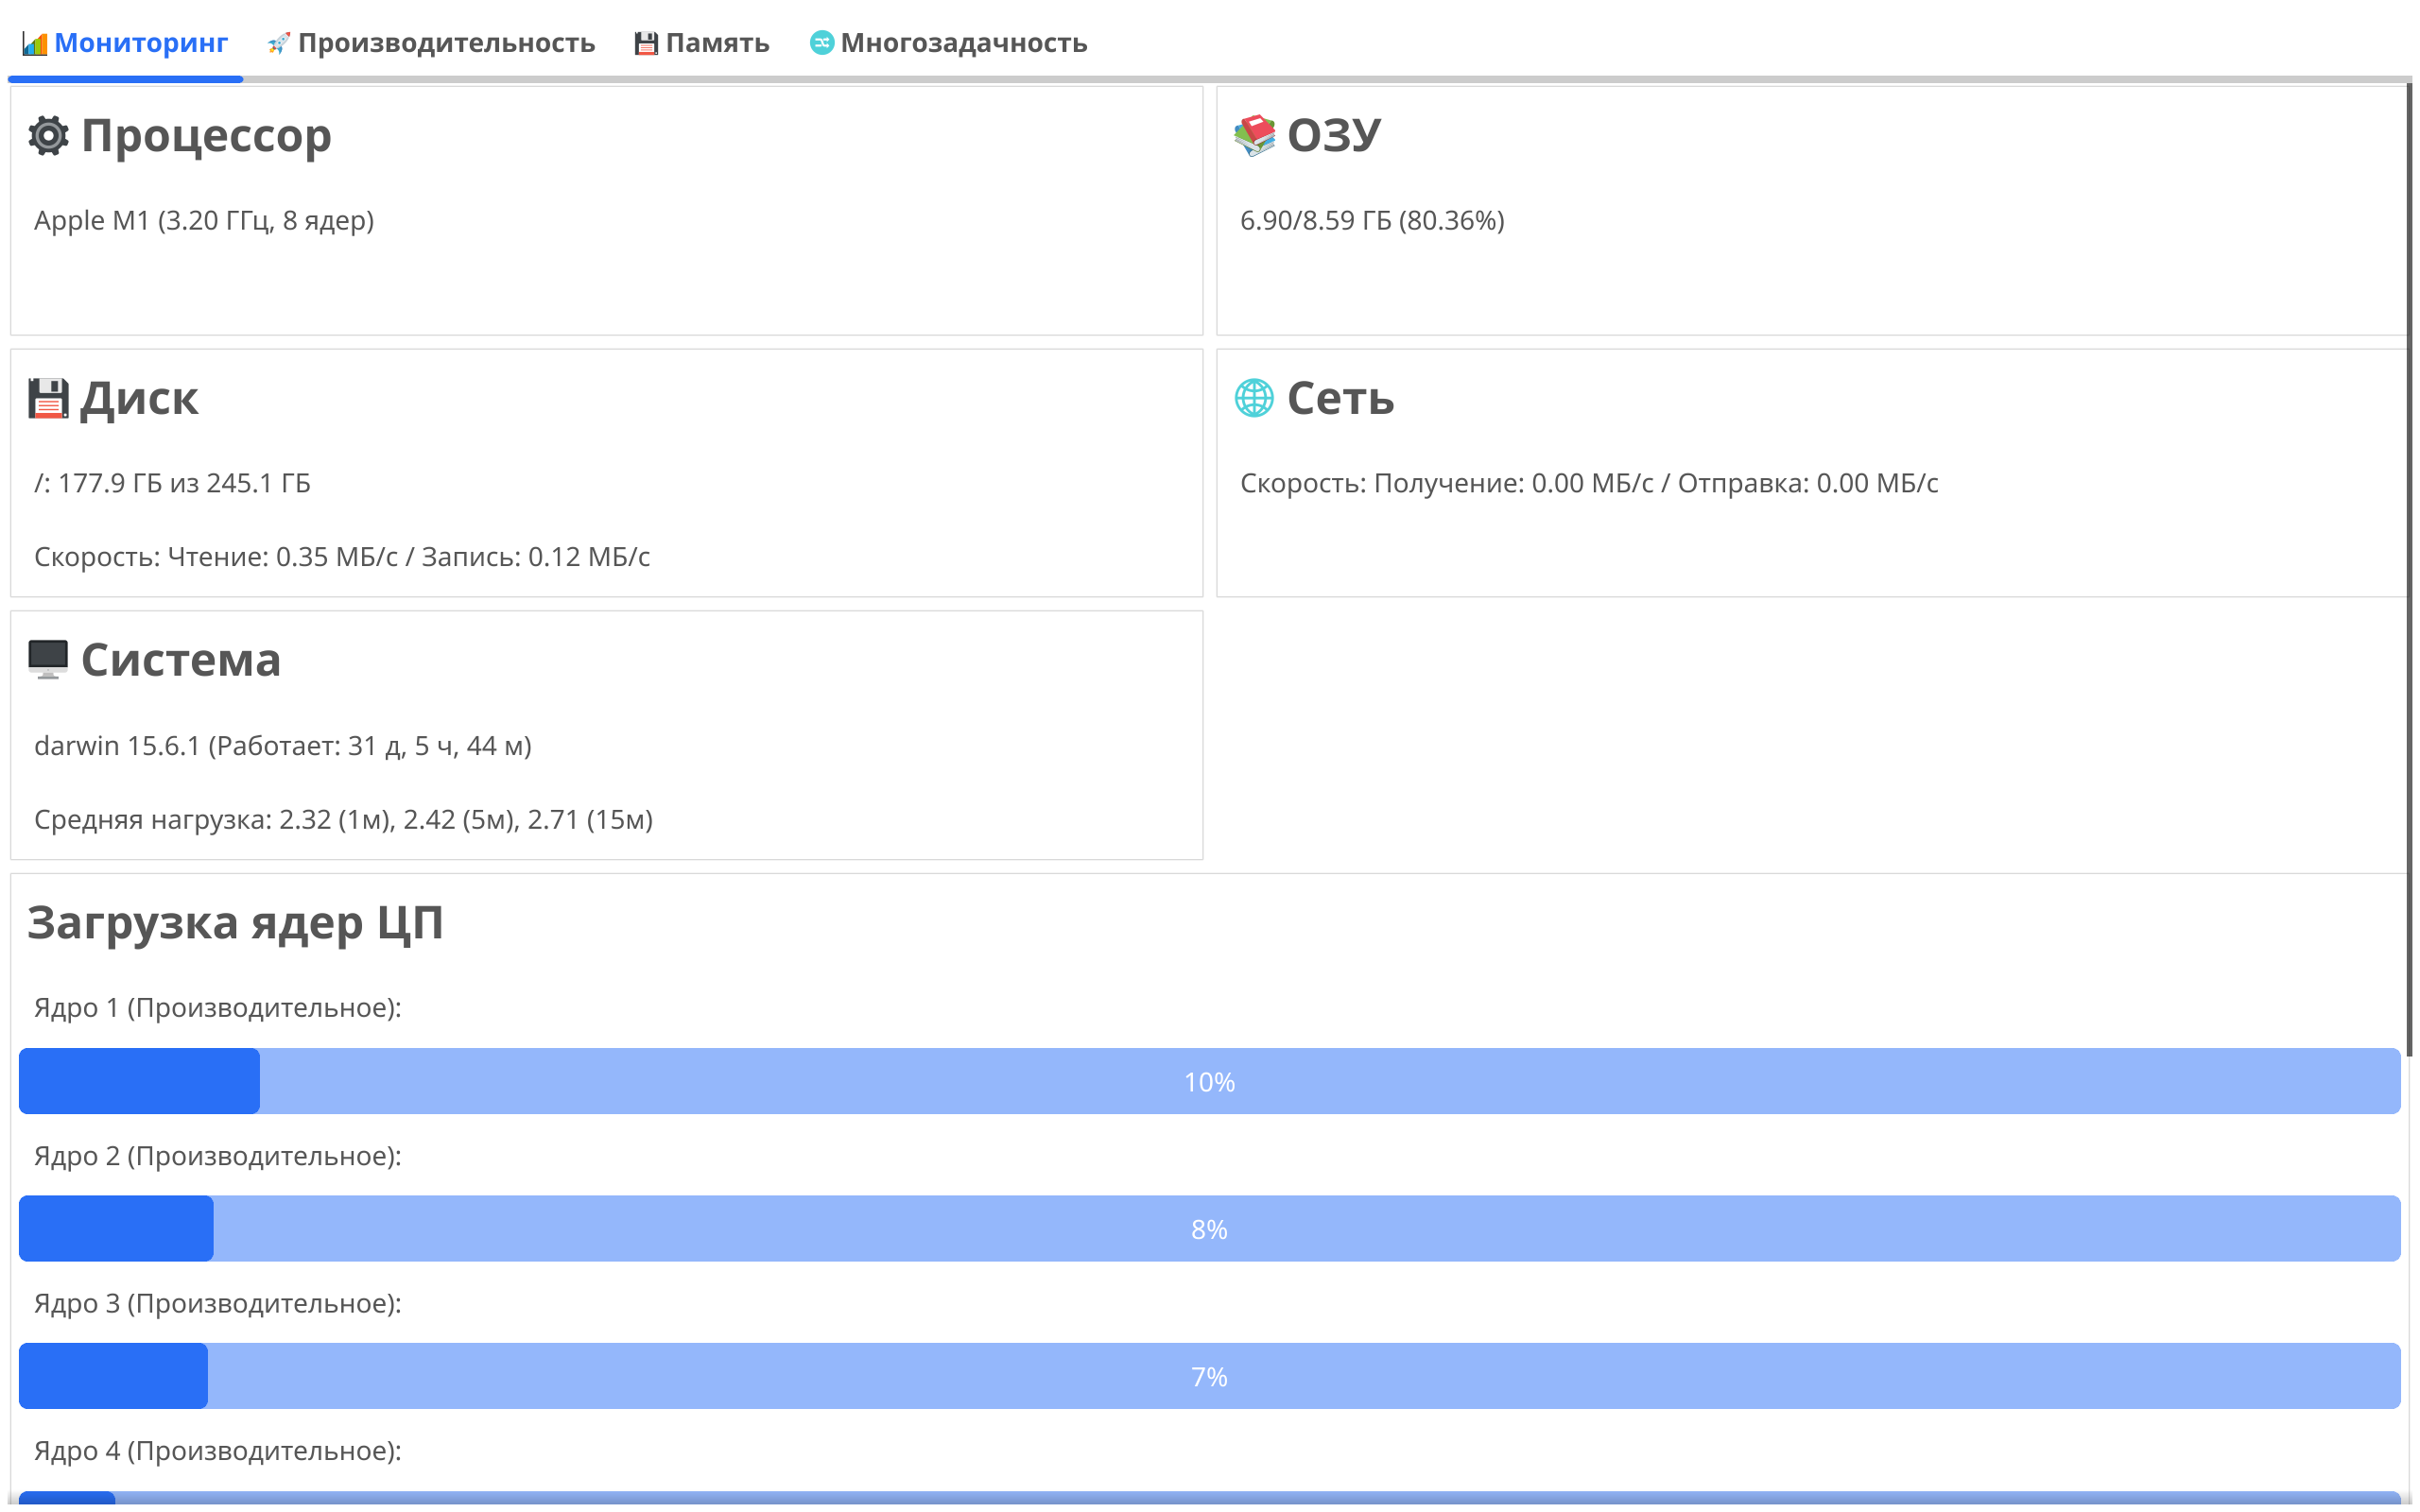
\includegraphics[width=0.9\textwidth]{main_window.png}\caption{Главное окно приложения с вкладкой «Мониторинг»}
\label{fig:main_window}
\end{figure}

\subsection{Панель мониторинга}

Панель мониторинга (\texttt{DashboardPanel}) — наиболее динамичная часть интерфейса. Ее ключевая особенность — фоновая горутина, которая с интервалом в 500 миллисекунд опрашивает модуль \texttt{profiling} и асинхронно обновляет виджеты. Информация сгруппирована в карточки (\texttt{widget.NewCard}) для логического разделения. Особого внимания заслуживает реализация отображения загрузки ядер ЦП. При инициализации панели определяется количество ядер и их тип (P-core/E-core для macOS). Затем для каждого ядра создается свой прогресс-бар, который обновляется в цикле.

\subsection{Панели тестирования}

Все три панели с тестами («Производительность», «Память», «Многозадачность») имеют схожую структуру, основанную на универсальном обработчике тестов \texttt{TestRunner}. Логика их работы заключается в следующем:
\begin{enumerate}
    \item При создании панели формируется список тестов. Для каждого теста определяется его название, описание и функция, реализующая его логику.
    \item На панели размещаются кнопка для запуска всех тестов и общий прогресс-бар.
    \item При нажатии на кнопку запускается горутина, которая итерируется по списку тестов и для каждого из них вызывает \texttt{TestRunner}. Это гарантирует, что интерфейс не будет заблокирован на время выполнения длительных вычислений.
    \item \texttt{TestRunner} многократно выполняет переданную ему функцию теста, собирает статистику (min, max, avg) и сообщает о прогрессе через специальный канал. Данные о прогрессе агрегируются и отображаются на общем прогресс-баре.
    \item По завершении каждого теста его результат форматируется и отображается в соответствующей карточке на панели.
\end{enumerate}

\begin{figure}[ht!]
\centering
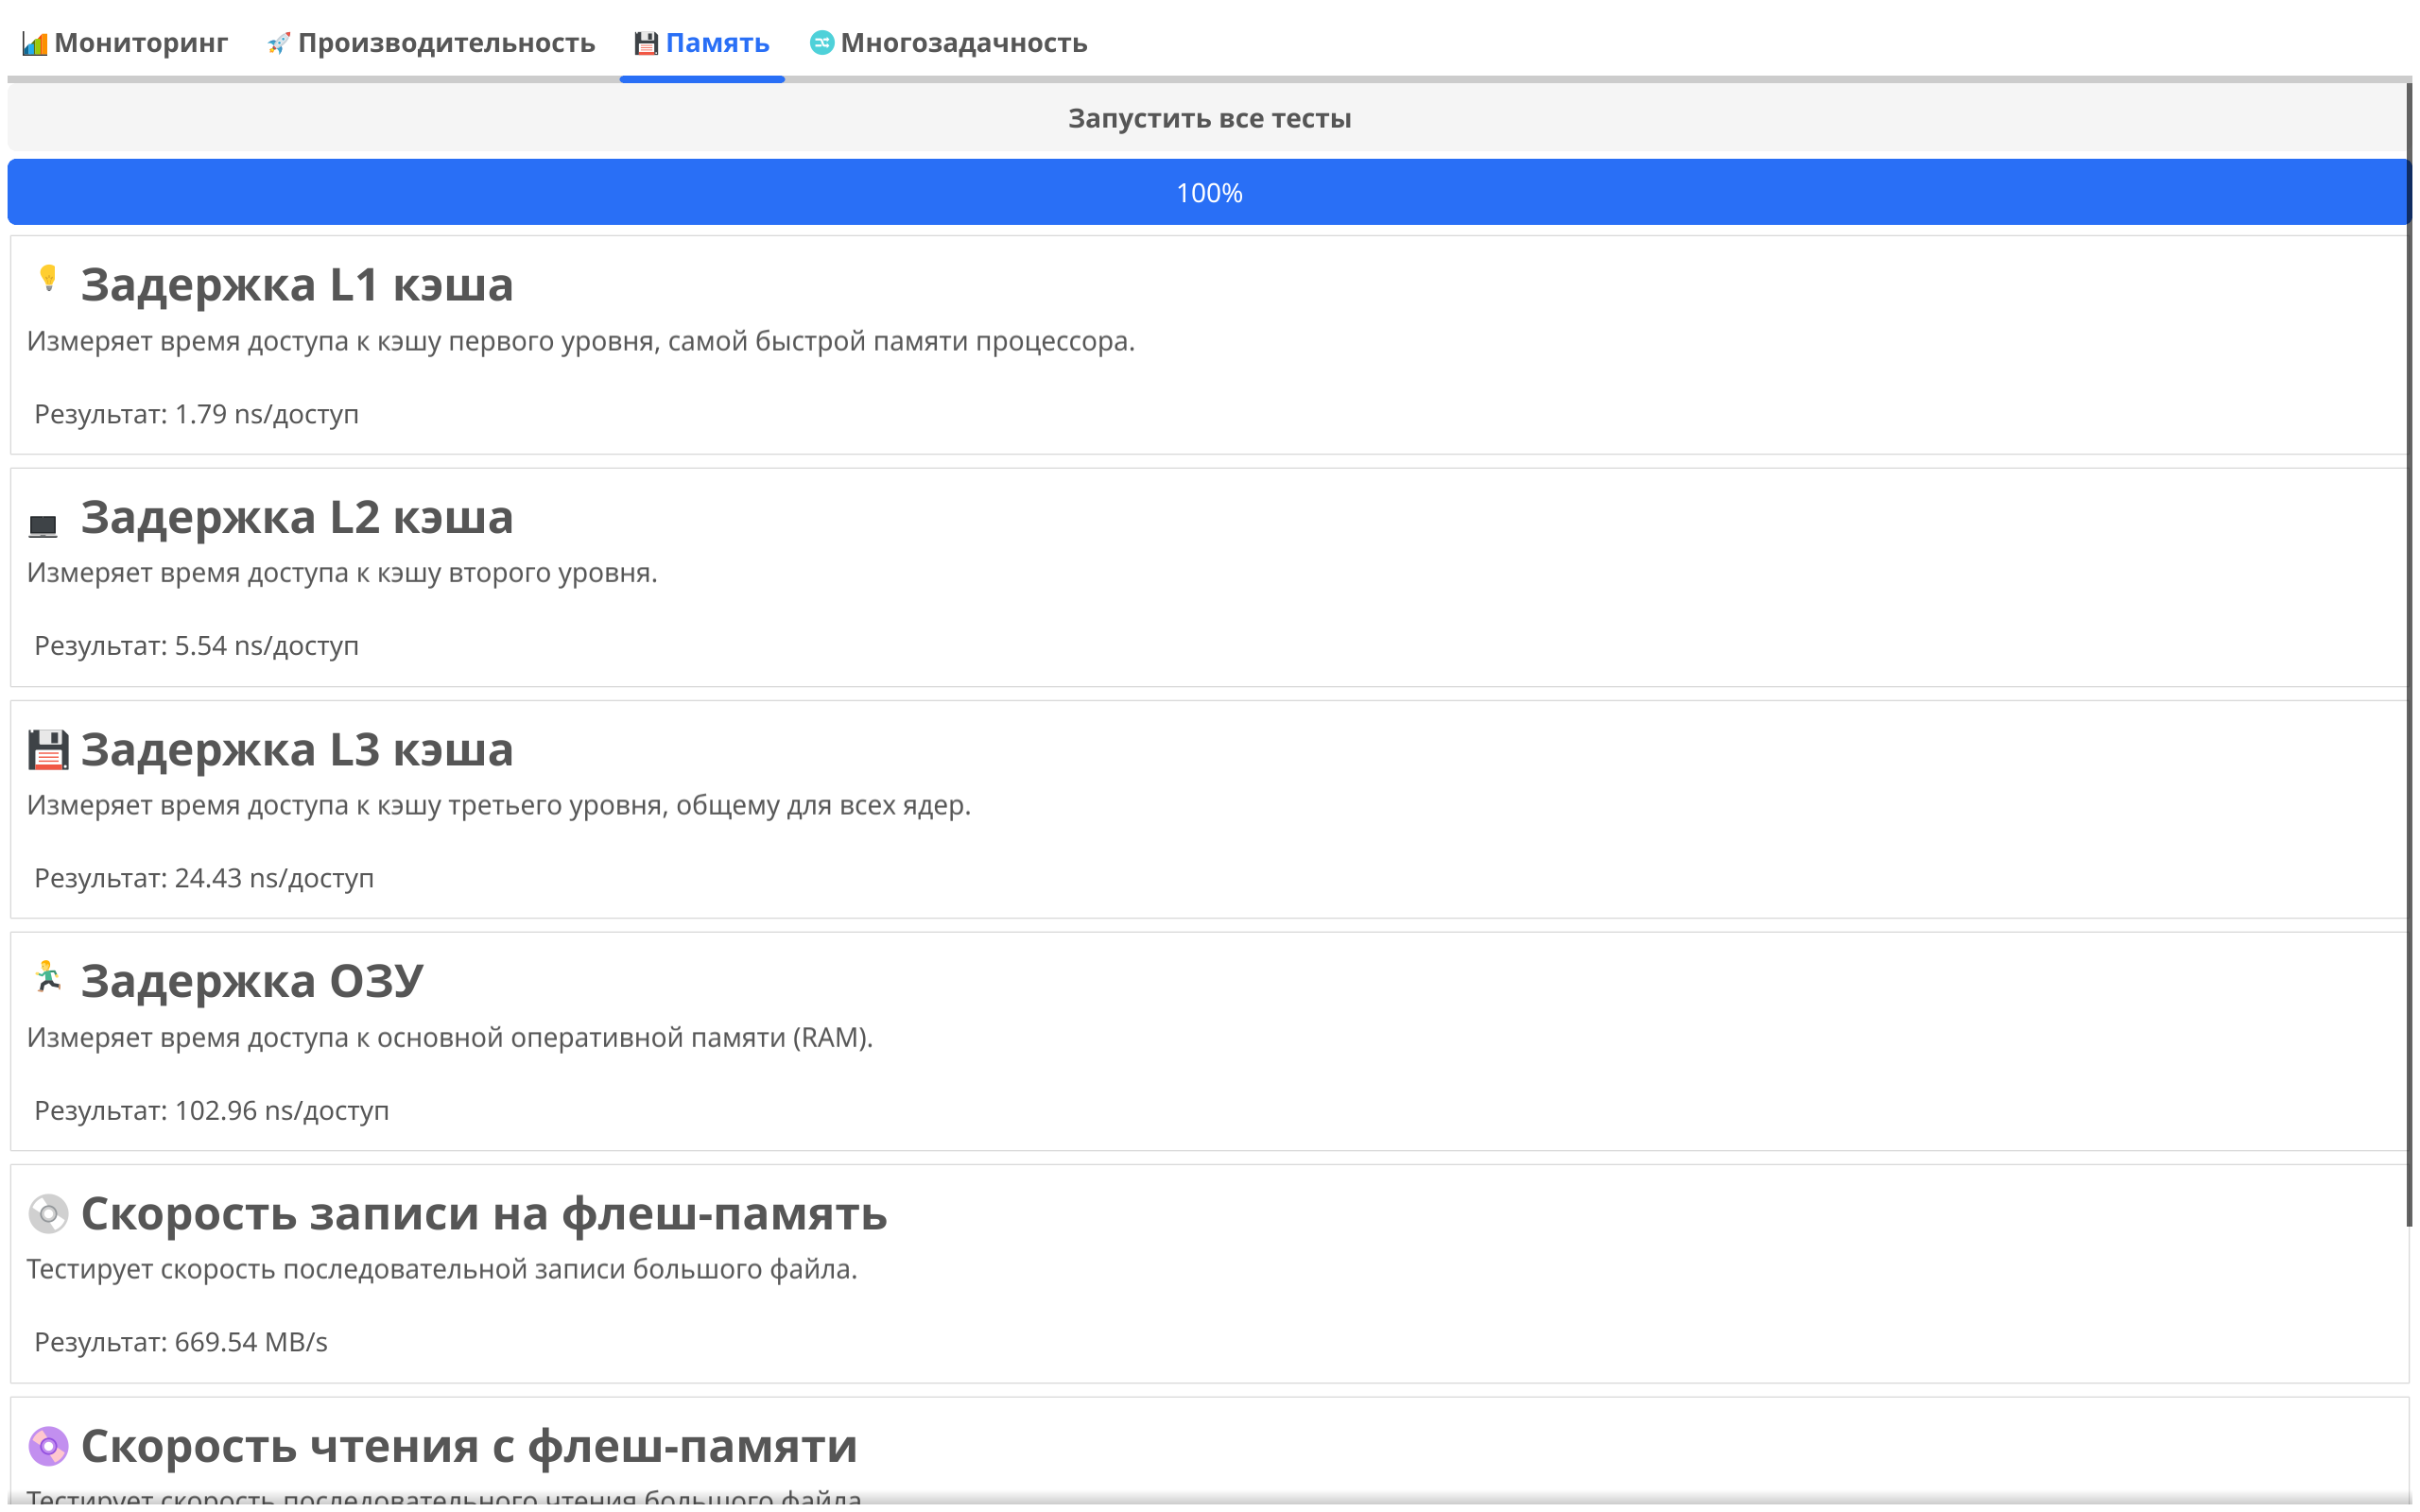
\includegraphics[width=0.9\textwidth]{memory_tests.png}\caption{Вкладка «Память» после завершения всех тестов}
\label{fig:memory_tests}
\end{figure}

\section{Реализация и результаты тестов}

\subsection{Тесты производительности ЦП}

\paragraph{Целочисленная арифметика.} Тест выполняет большое количество базовых операций (сложение, вычитание, умножение, деление) над 64-битными целочисленными переменными в цикле. Этот тест хорошо отражает базовую производительность процессора на задачах общего назначения.

\textbf{Результат:} в среднем \textbf{0.76 ns/op} (эквивалентно 1.31 млрд оп/с). Это означает, что процессор выполняет одну итерацию цикла (состоящую из 4-х операций) за очень малое время, что свидетельствует о высокой эффективности его конвейера.

\paragraph{Арифметика с плавающей запятой.} Аналогичный тест, но с использованием чисел с плавающей запятой двойной точности (\texttt{float64}).

\textbf{Результат:} в среднем \textbf{0.47 ns/op} (эквивалентно 2.14 млрд оп/с). Результат даже выше, чем у целочисленных операций, что говорит о чрезвычайно высокой производительности блока FPU (Floating-Point Unit) в тестируемом процессоре.

\subsection{Тесты иерархии памяти}

\paragraph{Задержка доступа.} Для этого теста используется алгоритм «погони за указателями» (pointer chasing), который позволяет измерить «чистую» задержку доступа к данным на разных уровнях иерархии памяти.

\textbf{Результаты:}
\begin{itemize}
    \item Задержка L1 кэша: \textbf{1.94 ns/доступ}
    \item Задержка L2 кэша: \textbf{5.57 ns/доступ}
    \item Задержка L3 кэша: \textbf{27.56 ns/доступ}
    \item Задержка ОЗУ: \textbf{99.46 ns/доступ}
\end{itemize}
Результаты наглядно демонстрируют огромную разницу в скорости: доступ к L1 почти в 3 раза быстрее, чем к L2, и в ~50 раз быстрее, чем к ОЗУ. Эти данные критически важны для оптимизации производительности: они показывают, что эффективное использование кэша (например, путем обработки данных небольшими блоками, помещающимися в кэш) может ускорить программу в десятки раз по сравнению с наивным алгоритмом, постоянно обращающимся в ОЗУ.

\paragraph{Пропускная способность ОЗУ.} Тест измеряет скорость, с которой процессор может читать или записывать большие объемы данных в оперативную память.

\textbf{Результаты:}
\begin{itemize}
    \item Пропускная способность чтения: \textbf{2890 МБ/с} (2.89 ГБ/с)
    \item Пропускная способность записи: \textbf{2800 МБ/с} (2.80 ГБ/с)
    \item Случайный доступ: \textbf{460 МБ/с} (0.46 ГБ/с)
\end{itemize}
Видно, что последовательный доступ значительно быстрее случайного (более чем в 6 раз), что наглядно демонстрирует работу аппаратного предсказателя (prefetcher) в контроллере памяти. Он пытается заранее загрузить в кэш данные, которые, по его предположению, скоро понадобятся. При последовательном доступе это работает идеально, при случайном — совершенно бесполезно. Низкая производительность случайного доступа является основным узким местом для таких приложений, как системы управления базами данных (СУБД).

\paragraph{Производительность флеш-накопителя.}
Тесты создают временный файл и измеряют скорость последовательной записи, последовательного чтения и случайного чтения.

\textbf{Результаты:}
\begin{itemize}
    \item Скорость записи: \textbf{612.63 МБ/с}
    \item Скорость чтения: \textbf{4943.87 МБ/с}
    \item Случайное чтение: \textbf{3644.44 МБ/с}
\end{itemize}
Высокие показатели чтения (почти 5 ГБ/с) свидетельствуют об использовании быстрого NVMe SSD накопителя, работающего через шину PCI Express. При этом скорость записи значительно ниже, что является типичной характеристикой для большинства твердотельных накопителей. Скорость случайного чтения также очень высока, что обеспечивает быстрый запуск приложений и загрузку системы.

\subsection{Тесты механизмов параллелизма}

\paragraph{Накладные расходы на создание горутин.} Тест показывает, насколько «дешево» для системы обходится создание одной горутины.

\textbf{Результат:} \textbf{408.60 ns/op}. Это подтверждает, что горутины являются чрезвычайно легковесным механизмом.

\paragraph{Производительность примитивов синхронизации.} Проводится сравнительный анализ производительности мьютекса (\texttt{sync.Mutex}) и атомарных операций (\texttt{atomic.AddInt64}) в условиях высокой конкуренции.

\textbf{Результаты:}
\begin{itemize}
    \item Блокировка мьютекса: \textbf{68.58 ns/op}
    \item Атомарные операции: \textbf{21.62 ns/op}
\end{itemize}
Результаты показывают, что для простых операций, таких как инкремент счетчика, атомарные операции более чем в 3 раза эффективнее. Это объясняется тем, что атомарная операция транслируется в одну специальную инструкцию процессора (например, `LOCK ADD`), тогда как захват и освобождение мьютекса требуют выполнения целой серии инструкций и потенциального обращения к ядру ОС для блокировки потока. Вывод: для простых модификаций разделяемых данных всегда следует предпочитать атомарные операции.

\paragraph{Производительность каналов и конвейеров.}
\begin{itemize}
    \item Пропускная способность каналов: \textbf{33.13 ns/op}
    \item Конвейерная обработка: \textbf{157.90 ns/op}
\end{itemize}
Время на пересылку данных через канал (33 ns) сопоставимо со стоимостью блокировки мьютекса, что показывает наличие определенных накладных расходов на синхронизацию внутри реализации каналов. Результат конвейера (158 ns) примерно в 5 раз выше, что логично, так как данные проходят через несколько стадий (каналов) последовательно. Этот тест демонстрирует, что при проектировании высоконагруженных параллельных систем необходимо минимизировать количество пересылок данных между горутинами.
